\section{Conception Matérielle}
Pour mettre en oeuvre les différentes parties du projet combinatoires et séquentielles, nous avons du passer par des étapes d'analyses comportementales de chaque blocs à réaliser pour ainsi créer des composants simples pouvant être utilisés à la composition de fonctions plus complexes plus tard. L'implémentation de chaque composants a été réalisée grâce au langage VHDL sur le logiciel de développement Quartus.

Ainsi nous avons réalisé différentes "boîtes" de composants simples pour réaliser des fonctions entières, et plus complexes, contenant les blocs simples.

\subsection{Réalisation fonction simple - Gestion anémomètre}
La fonction réalisant l'acquisition de la vitesse du vent (0 à 250 Km/h) se fait à l'aide d'un anémomètre qui sert de transducteur convertissant la vitesse du vent en fréquence variable (0 à 250 Hz). 
\vspace{0.5cm}\\
Le composant doit fonctionner en deux modes :
\begin{enumerate}
    \item Mode continu, dans ce mode le système actualise l'acquisition toutes les secondes de la vitesse du vent. Pour cela l'entrée "Continu" doit être à 1. 
    \item Mode mono-coup, dans ce mode le système effectue qu'une seule acquisition lorsque "Start/Stop" est activé. Une fois "data\_valide" envoyé le système remet les entrées "Start/Stop" et "data\_valide" à zéro après une acquisition et attend la prochaine entrée "Start/Stop".
\end{enumerate}
\vspace{0.5cm}
La figure 3 représente la décomposition des composants utilisés pour la réalisation du bloc "Captage force vent". 

\begin{figure}[h]
    \begin{center}
      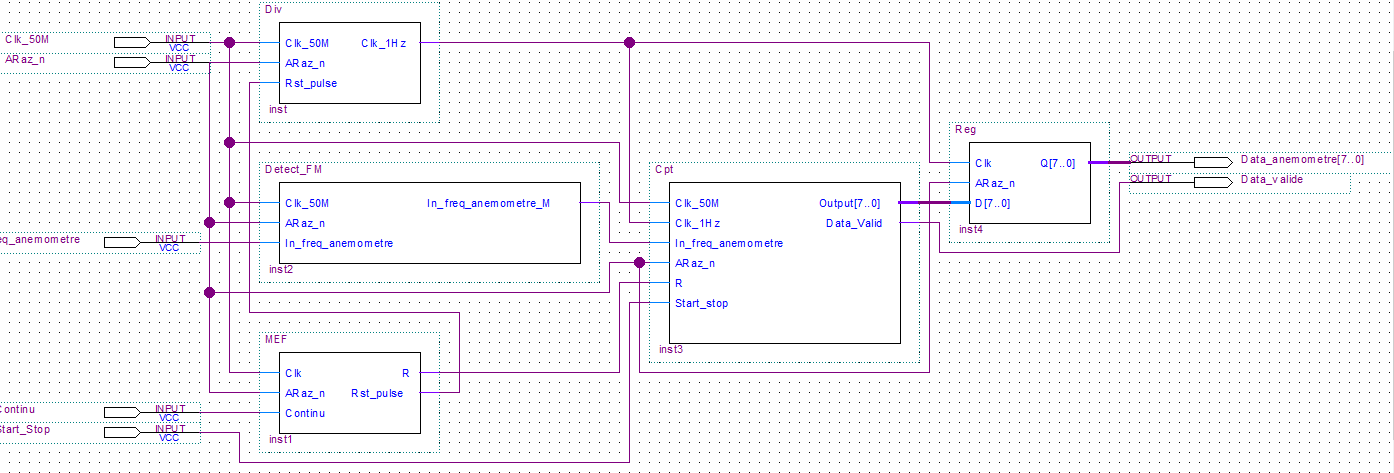
\includegraphics[width=\textwidth]{images/captation.png}
      \caption{Diagramme fonctionnel du circuit "Captation vitesse vent"}
    \end{center}
  \end{figure}

  Le composant "Div" fournit une horloge de 1 Hz à partir de l'horloge 50 MHz donnée par la clock du FPGA. L'horloge de 1 Hz sera utilisée pour l'acquisition de la fréquence de l'anémomètre toutes les secondes.

\newpage

  Le deuxième composant "Detect\_FM" est en charge de détecter les fronts montants sortant de l'anémomètre pour transformer la fréquence générée en Hertz en une donnée interprétable par le composant "Cpt".\\\newline

  Le composant "Cpt" va permettre de récupérer la quantité de fronts montants comptés par le composant "Detect\_FM", toutes les secondes quand le composant sera en mode continue et une seule fois lors du mode mono-coup.\\\newline

  Le composant "Reg" permettant de stocker la valeur de la fréquence convertie dans un registre ce qui va permettre de venir traiter ou effectuer des calculs une fois celle-ci acquise (ici dans le MCU qui sera réalisé prochainement).\\\newline

  Le composant "MEF" est chargé de gérer le mode de fonctionnement du circuit, ce qui permet à ce bloc fonctionnel de savoir quand il doit être remis à zéro ou savoir quand il est en mode "Continu" ou "Mono-coup".\vspace{1cm}
  \begin{figure}[h]
    \begin{center}
      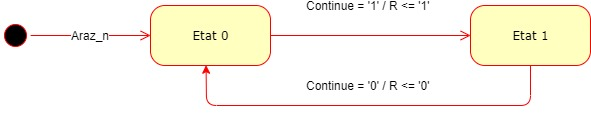
\includegraphics[width=\textwidth]{images/MEF_anemo.jpg}
      \caption{Machine à états Gestion anémomètre}
    \end{center}
  \end{figure}

Au projet, une partie interface Avalon a été ajoutée permettant l'implémentation et l'interfaçage des fonctions entre la partie NIOS II et la partie matérielle FPGA. 
  \newpage

  \subsection{Réalisation fonction complexe - Gestion vérin}

  La fonction réalisant le mouvement de la barre franche est réalisé avec le circuit vérin. Ce circuit est composé de 3 fonctions principales qui vont permettre le pilotage du vérin qui contrôle la barre franche du voilier :\vspace{0.5cm}
\begin{enumerate}
    \item Une gestion d'un signal PWM effectué par le process "PWM" qui va permettre de faire sortir ou rentrer le vérin en fonction d'une fréquence et le rapport cyclique. 
    \item Un contrôle des butées réalisé par le process "Gestion\_Butée" qui sous certaines conditions fixées dans la partie logicielle du projet fera l'avance ou le recul du vérin jusqu'à celles-ci.
    \item Une machine à états pour la gestion du convertisseur MCP3201 12 bits rendant possible le déplacement du vérin dans un sens puis dans un autre.
    \item Une partie interface Avalon est ajouté au projet pour créer le lien entre la partie logicielle et la partie matérielle du FPGA/NIOS II.
\end{enumerate} 

  \begin{figure}[h]
    \begin{center}
      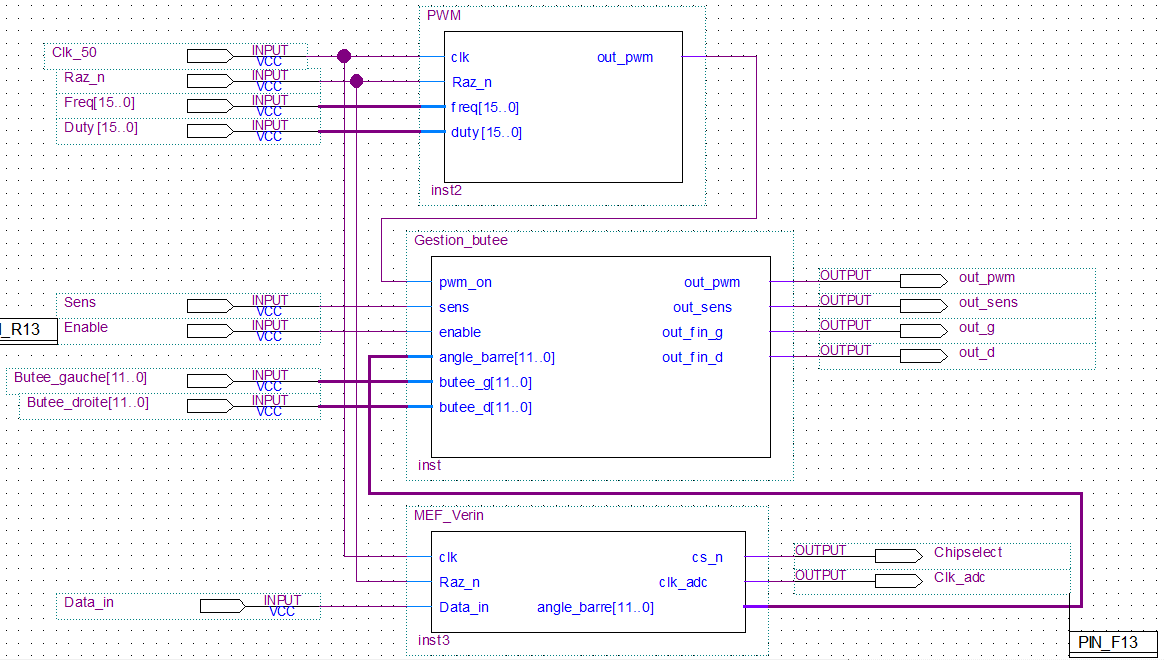
\includegraphics[width=\textwidth]{images/verin.png}
      \caption{Diagramme fonctionnel du circuit "Actionnement Barre"}
    \end{center}
  \end{figure}

\newpage 

La machine à états ci-dessous décrit le comportement du bloc Gestion vérin permettant ainsi de gérer le pilotage du convertisseur AN MCP3201 qui va mémoriser la donnée "angle\_barre" pour ensuite l'écrire sur le bus du NIOS II puis dans des régistres.
\vspace{1cm}
  \begin{figure}[h]
    \begin{center}
      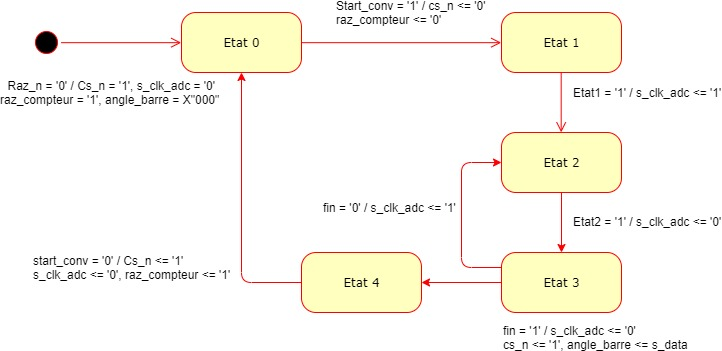
\includegraphics[width=\textwidth]{images/MEF_verin.jpg}
      \caption{Machine à états Gestion vérin}
    \end{center}
  \end{figure}

  \newpage

  \subsection{Réalisation interfaces Avalon}

La création d'une interface processeur et matériel programmable est nécessaire au bon fonctionnement du projet. Altera a développé un bus informatique appelé bus "Avalon" destiné à l'implémentation matériel/composants sur FPGA. Il va permettre l'interconnexion entre le processeur NIOS II (réalisé à l'aide de SOPC builder) et les périphériques des différents composants que nous avons créé ultérieurement.\\
\newline
Pour réaliser cette interface il a fallut respecter le cahier des charges donné en début de projet pour chaque interfaces, qui correspondent à des circuits combinatoires/séquentiels utilisés pour l'écriture et la lecture du bus (Address, read, write, chip select...). Ci-dessous sont représentés les différents circuits que nous avons implémenté au projet.\\
\newline
La première interface correspond à la fonction Anémomètre.
\begin{figure}[h]
  \begin{center}
    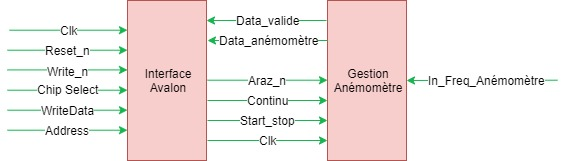
\includegraphics[width=0.8\textwidth]{images/avalon_anemo.jpg}
    \caption{Interface Avalon Gestion anémomètre}
  \end{center}
\end{figure}\\
\newline
La deuxième interface correspond à la fonction Gestion vérin.

\begin{figure}[h]
  \begin{center}
    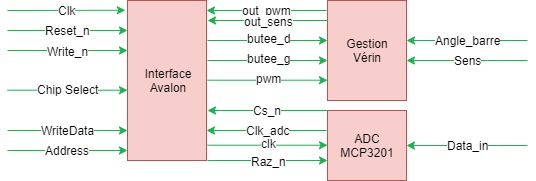
\includegraphics[width=0.8\textwidth]{images/avalon_verin.jpg}
    \caption{Interface Avalon Gestion vérin}
  \end{center}
\end{figure}